\section{Задание 4. Аппроксимация RBF-сетью}

\subsection{Постановка задачи}

Используя те же данные варианта 7, выполнить аппроксимацию функции с помощью RBF-сети (сеть с радиальными базисными функциями). Требуется:
\begin{itemize}
    \item реализовать модель на языке Python;
    \item использовать MSE функцию потерь и градиентный спуск (Стратегия 2);
    \item построить кривую обучения;
    \item вычислить невязки на каждом объекте;
    \item построить модельную поверхность и линии уровня вместе с точками данных;
    \item записать аналитический вид модели.
\end{itemize}

\subsection{Математическая модель}

RBF-сеть --- двухслойная нейронная сеть, выход которой является линейной комбинацией гауссовых радиальных функций:

\begin{equation}\label{eq:rbf}
    z(\mathbf{x}) = b + \sum_{j=1}^{M} w_j \cdot \exp\left(-\frac{\|\mathbf{x} - \mathbf{c}_j\|^2}{2\sigma_j^2}\right),
\end{equation}

где $M = 2$ --- число нейронов скрытого слоя; $\mathbf{c}_j = (c_{j1}, c_{j2})$ --- центры; $\sigma_j$ --- ширины (размах); $w_j$ --- веса; $b$ --- смещение (bias).

Вектор параметров: $\mathbf{p} = (b, w_1, w_2, \mathbf{c}_1, \mathbf{c}_2, \sigma_1, \sigma_2)$ --- всего $1 + 2 + 4 + 2 = 9$ параметров.

\subsection{Алгоритм обучения}

\textbf{Этап 1: Инициализация центров методом K-средних.}

Центры инициализируются кластеризацией входных точек $(x, y)$ на $M=2$ кластера. Результаты K-средних:
\begin{itemize}
    \item $\mathbf{c}_1 = (1.5550, 1.5400)$ --- центр первого кластера (ближе к началу координат);
    \item $\mathbf{c}_2 = (3.9900, 3.9133)$ --- центр второго кластера (ближе к пику).
\end{itemize}

Ширины вычисляются как половина расстояния между центрами: $\sigma_1 = \sigma_2 = 0.5 \cdot \|\mathbf{c}_1 - \mathbf{c}_2\| = 1.7001$.

Веса $w_j$ инициализируются случайно из $\mathcal{N}(0, 0.5^2)$, $b = 0$.

\textbf{Этап 2: Градиентный спуск.}

Функция потерь: $L = \frac{1}{N}\sum_{i=1}^{N}(z(\mathbf{x}_i) - z_i)^2$.

Частные производные по всем параметрам (аналитические выражения для градиентного спуска):
\begin{align}
    \frac{\partial L}{\partial w_j} &= \frac{2}{N}\sum_{i=1}^{N} (z(\mathbf{x}_i) - z_i) \cdot \phi_j(\mathbf{x}_i), \label{eq:grad_w}\\
    \frac{\partial L}{\partial b} &= \frac{2}{N}\sum_{i=1}^{N} (z(\mathbf{x}_i) - z_i), \label{eq:grad_b}\\
    \frac{\partial L}{\partial \sigma_j} &= \frac{2}{N}\sum_{i=1}^{N} (z(\mathbf{x}_i) - z_i) \cdot w_j \cdot \phi_j(\mathbf{x}_i) \cdot \frac{\|\mathbf{x}_i - \mathbf{c}_j\|^2}{\sigma_j^3}, \label{eq:grad_sigma}\\
    \frac{\partial L}{\partial \mathbf{c}_j} &= \frac{2}{N}\sum_{i=1}^{N} (z(\mathbf{x}_i) - z_i) \cdot w_j \cdot \phi_j(\mathbf{x}_i) \cdot \frac{\mathbf{x}_i - \mathbf{c}_j}{\sigma_j^2}, \label{eq:grad_c}
\end{align}
где $\phi_j(\mathbf{x}) = \exp\left(-\|\mathbf{x} - \mathbf{c}_j\|^2 / (2\sigma_j^2)\right)$ --- активация $j$-го нейрона.

Параметры обучения: скорость обучения $\eta = 0.1$, число эпох $= 500$.

\subsection{Кривая обучения}

\begin{figure}[H]
    \centering
    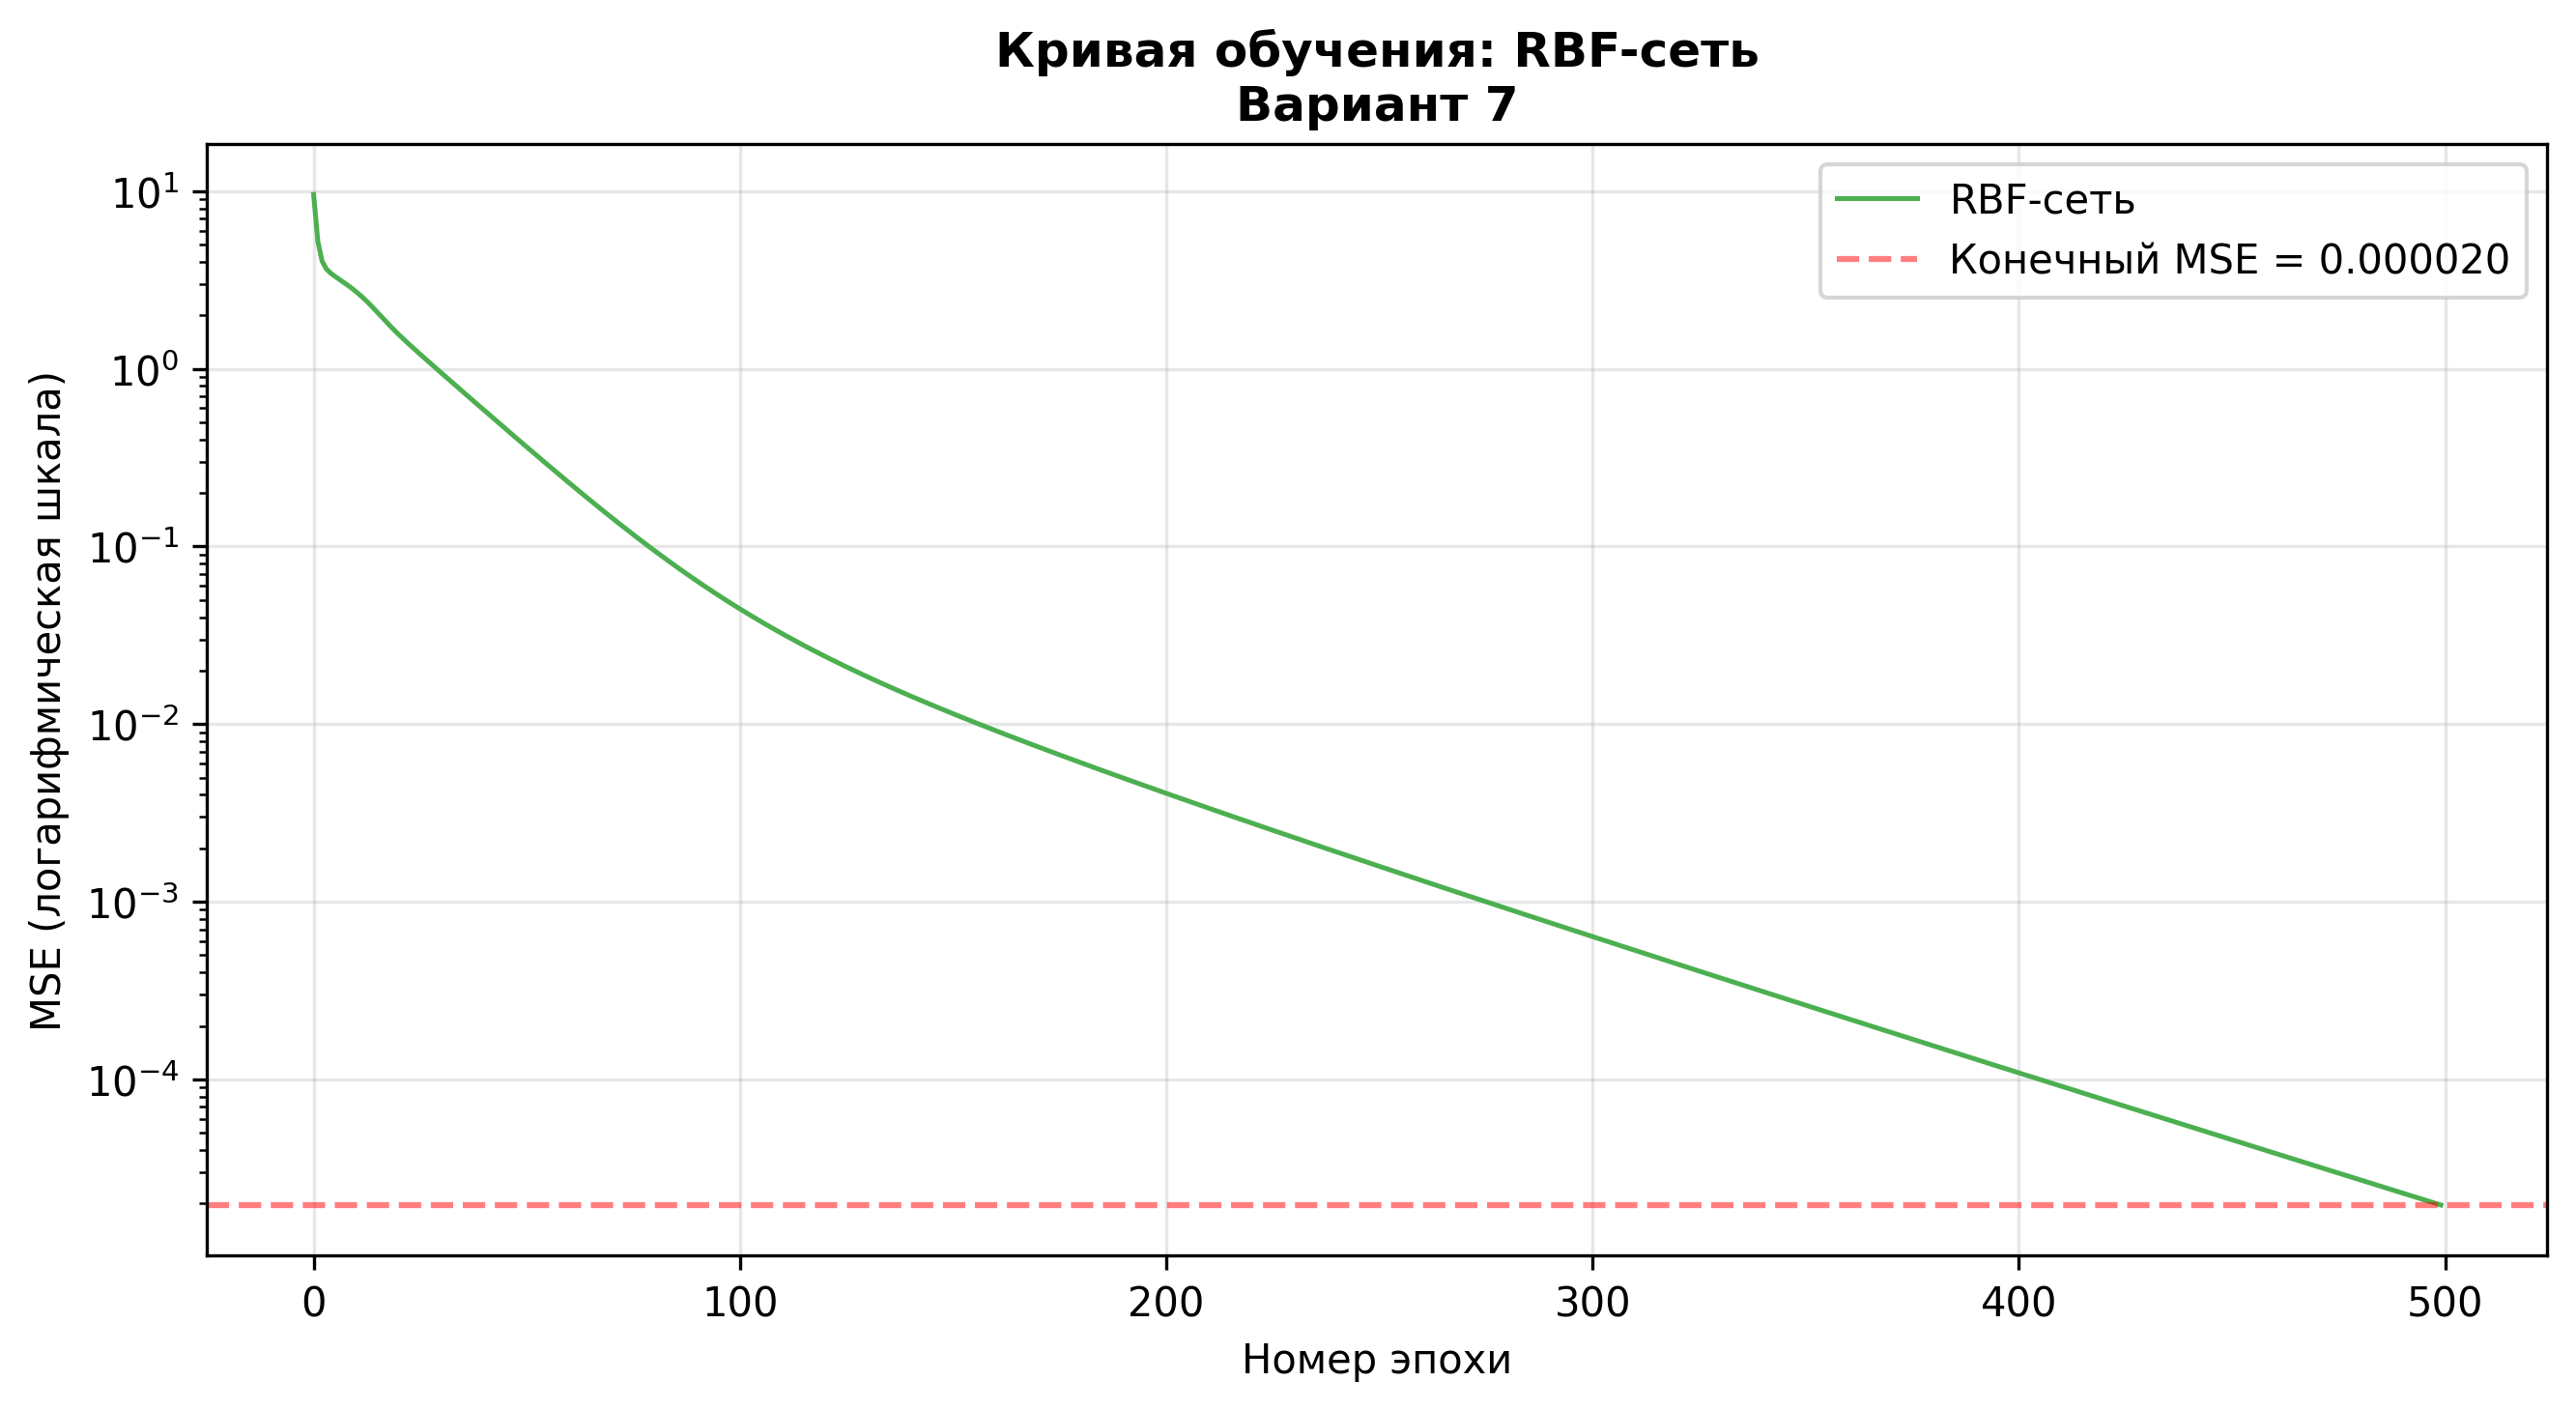
\includegraphics[width=0.85\textwidth]{pic/rbf_learning_curve.png}
    \caption{Кривая обучения RBF-сети (логарифмическая шкала)}
    \label{fig:rbf_learning}
\end{figure}

На рис.~\ref{fig:rbf_learning} показана динамика MSE в процессе градиентного спуска. Начальное значение MSE = 9.588, конечное --- 0.000019. Обучение сходится быстро: уже после $\sim 50$ эпох MSE падает ниже 0.1. После 300 эпох лосс практически стабилизируется.

\subsection{Результаты}

\begin{table}[H]
    \centering
    \caption{Оптимальные параметры RBF-сети}
    \label{tab:rbf_params}
    \begin{tabular}{|c|c|c|c|c|}
        \hline
        \textbf{Нейрон} & \textbf{Вес $w_j$} & \textbf{Центр $c_{j1}$} & \textbf{Центр $c_{j2}$} & \textbf{Ширина $\sigma_j$} \\
        \hline
        1 & -0.0060 & 1.5805 & 1.5606 & 1.7727 \\
        2 & 5.8173 & 3.3015 & 3.4716 & 1.0503 \\
        \hline
        \multicolumn{5}{|c|}{Смещение $b = 0.2456$} \\
        \hline
    \end{tabular}
\end{table}

\subsection{Аналитический вид модели}

\begin{equation}\label{eq:rbf_result}
    \begin{aligned}
        z(x,y) = 0.2456 &- 0.0060 \cdot \exp\left(-\frac{(x - 1.5805)^2 + (y - 1.5606)^2}{2 \cdot 1.7727^2}\right) \\
                         &+ 5.8173 \cdot \exp\left(-\frac{(x - 3.3015)^2 + (y - 3.4716)^2}{2 \cdot 1.0503^2}\right).
    \end{aligned}
\end{equation}

Анализ модели показывает:
\begin{itemize}
    \item \textbf{Нейрон 2} (вес $w_2 \approx 5.82$, центр $(3.30, 3.47)$, $\sigma_2 = 1.05$) моделирует основной пик. Его центр близок к центру пика данных.
    \item \textbf{Нейрон 1} (вес $w_1 \approx -0.006$) практически не влияет на выход --- его вес пренебрежимо мал.
    \item \textbf{Смещение} $b = 0.2456$ близко к фоновому уровню данных.
\end{itemize}

RBF-сеть фактически свела задачу к одной доминирующей гауссиане, что согласуется с результатами задания 1.

\subsection{Таблица невязок}

\begin{table}[H]
    \centering
    \caption{Невязки RBF-сети}
    \label{tab:rbf_residuals}
    \begin{tabular}{|c|c|c|c|c|c|}
        \hline
        \textbf{Точка} & \textbf{$x$} & \textbf{$y$} & \textbf{$z_{факт}$} & \textbf{$z_{модель}$} & \textbf{Невязка} & \textbf{Кв. невязки} \\
        \hline
        0 & 1.10 & 1.10 & 0.29 & 0.2906 & $5.6 \times 10^{-4}$ & $3.1 \times 10^{-7}$ \\
        1 & 2.01 & 1.98 & 1.24 & 1.2365 & $-3.5 \times 10^{-3}$ & $1.2 \times 10^{-5}$ \\
        2 & 3.01 & 2.85 & 4.94 & 4.9407 & $7.2 \times 10^{-4}$ & $5.2 \times 10^{-7}$ \\
        3 & 3.86 & 3.99 & 4.72 & 4.7157 & $-4.3 \times 10^{-3}$ & $1.9 \times 10^{-5}$ \\
        4 & 5.10 & 4.90 & 0.77 & 0.7780 & $8.0 \times 10^{-3}$ & $6.5 \times 10^{-5}$ \\
        \hline
    \end{tabular}
\end{table}

MSE $= 1.93 \times 10^{-5}$, RMSE $= 4.39 \times 10^{-3}$. Невязки малы, модель хорошо описывает данные.

\subsection{Визуализация}

\begin{figure}[H]
    \centering
    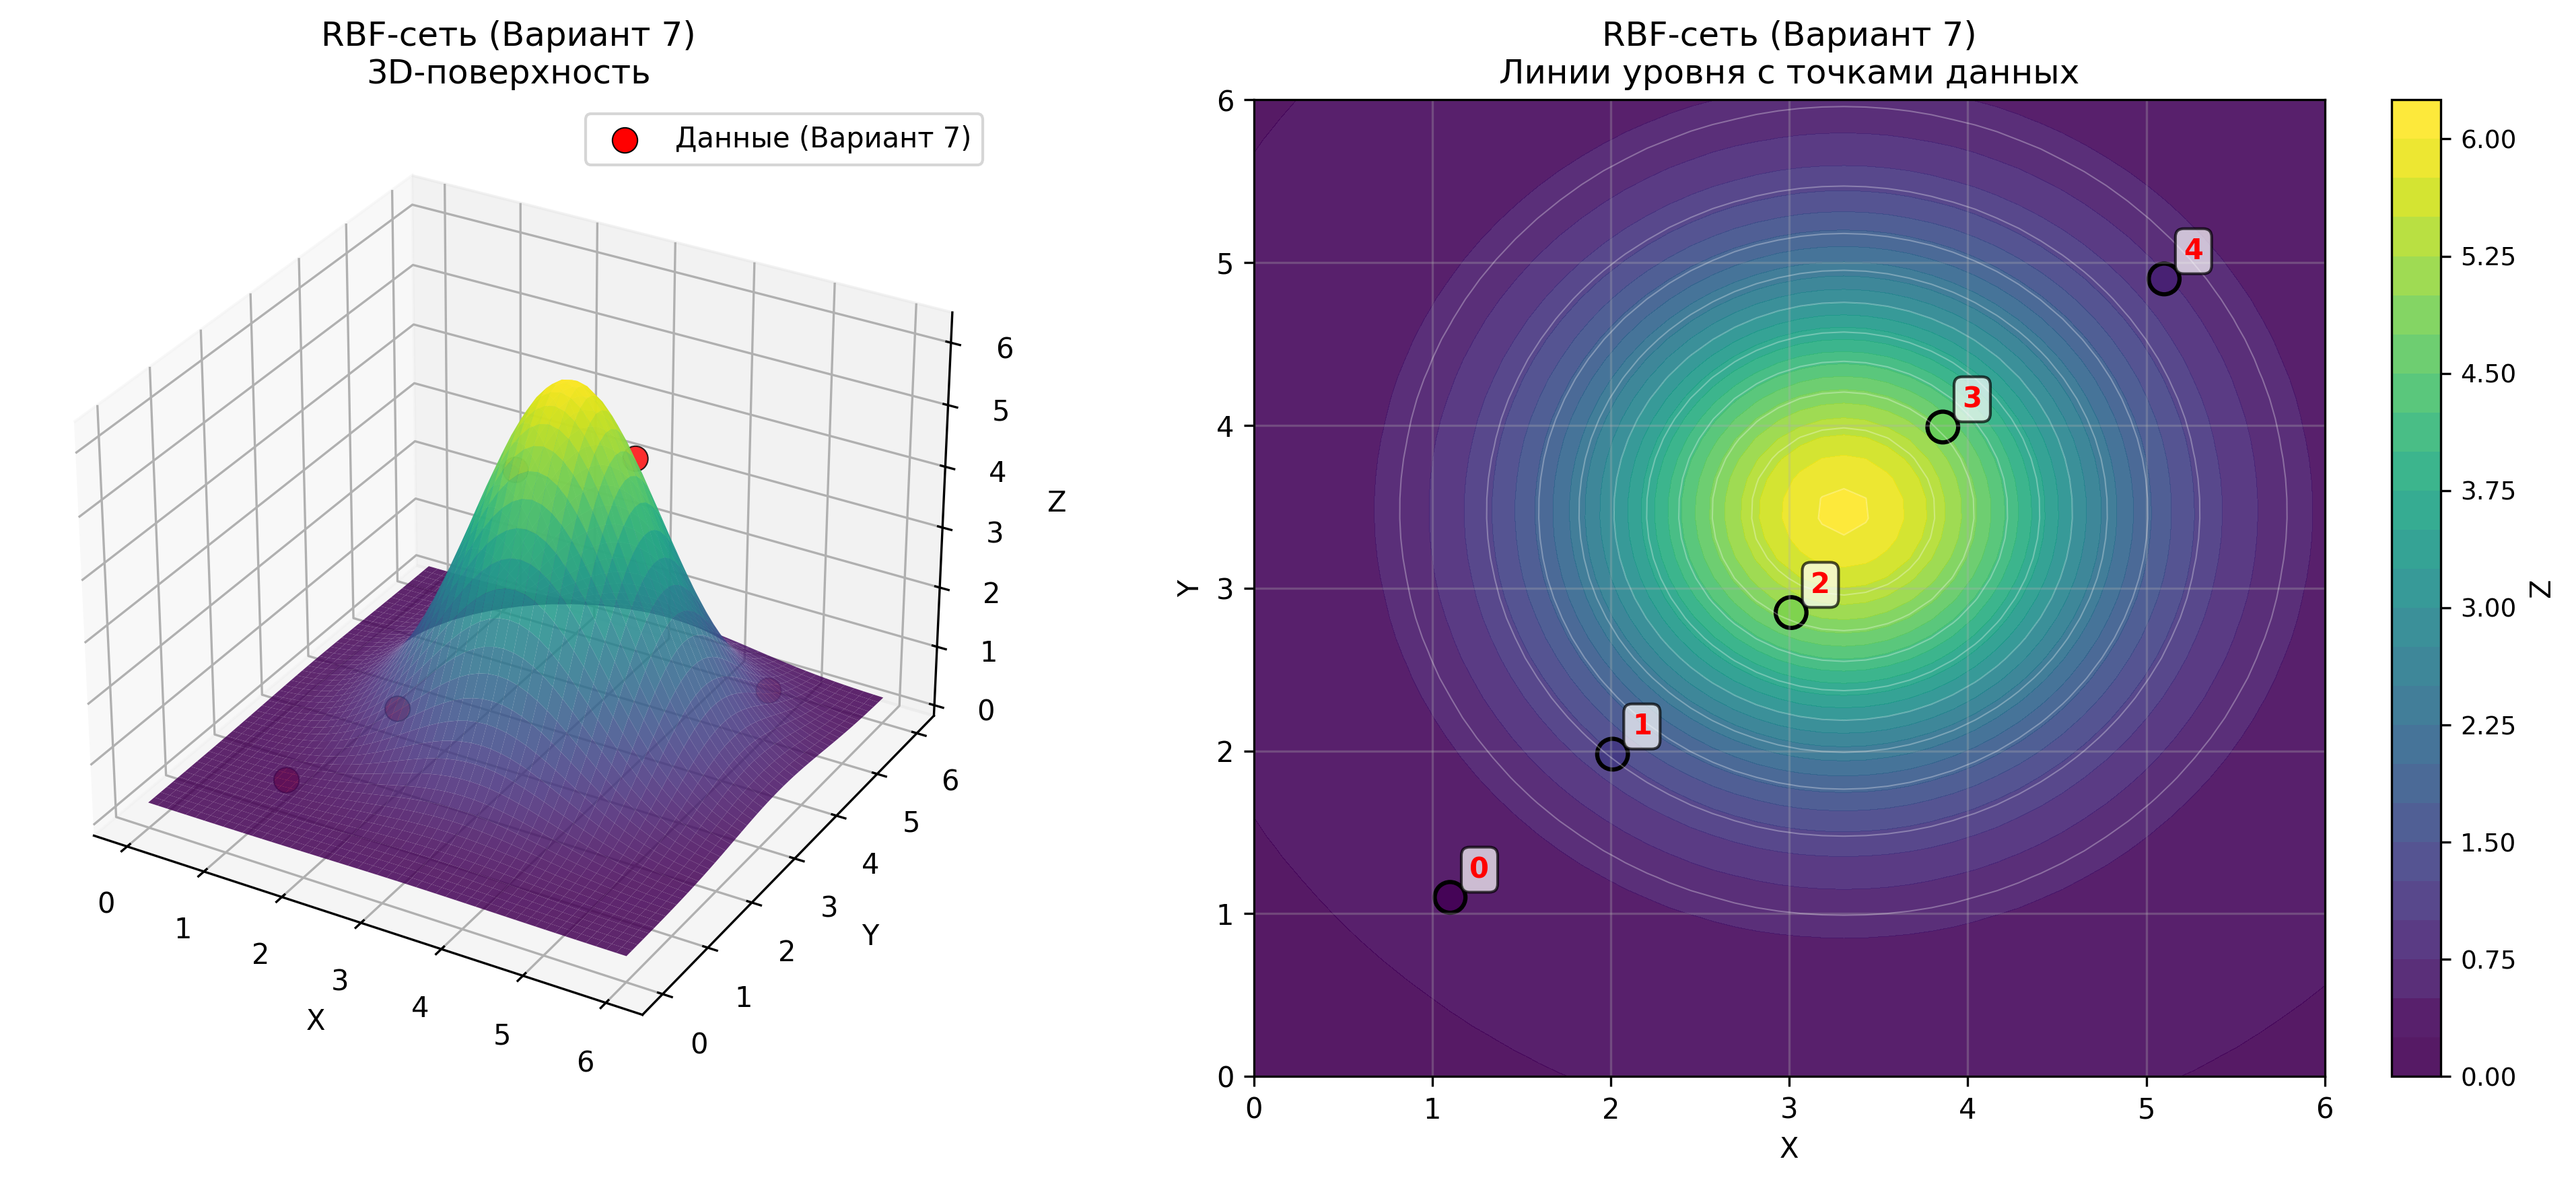
\includegraphics[width=\textwidth]{pic/rbf_model.png}
    \caption{RBF-сеть: 3D-поверхность (слева) и линии уровня с точками данных (справа)}
    \label{fig:rbf_model}
\end{figure}

Поверхность RBF-сети на рис.~\ref{fig:rbf_model} визуально неотличима от гауссовой модели. Она проходит через все экспериментальные точки и имеет гладкую колоколообразную форму.

\subsection{Сравнительный анализ трёх методов}

\begin{table}[H]
    \centering
    \caption{Сводная таблица результатов}
    \label{tab:comparison}
    \begin{tabular}{|c|c|c|c|c|c|}
        \hline
        \textbf{Точка} & \textbf{$z_{факт}$} & \textbf{Гауссиана} & \textbf{Параболоид} & \textbf{RBF-сеть} \\
        \hline
        0 & 0.29 & 0.2900 & -0.3753 & 0.2906 \\
        1 & 1.24 & 1.2400 & 2.7546 & 1.2365 \\
        2 & 4.94 & 4.9400 & 4.3267 & 4.9407 \\
        3 & 4.72 & 4.7200 & 4.1611 & 4.7157 \\
        4 & 0.77 & 0.7700 & 1.1524 & 0.7780 \\
        \hline
    \end{tabular}
\end{table}

\begin{table}[H]
    \centering
    \caption{Сравнение MSE и RMSE}
    \label{tab:mse_comp}
    \begin{tabular}{|l|c|c|c|}
        \hline
        \textbf{Метод} & \textbf{Параметров} & \textbf{MSE} & \textbf{RMSE} \\
        \hline
        Гауссиана & 7 & $2.27 \times 10^{-10}$ & $1.51 \times 10^{-5}$ \\
        Параболоид & 6 & 0.7142 & 0.8451 \\
        RBF-сеть & 9 & $1.93 \times 10^{-5}$ & $4.39 \times 10^{-3}$ \\
        \hline
    \end{tabular}
\end{table}

\begin{figure}[H]
    \centering
    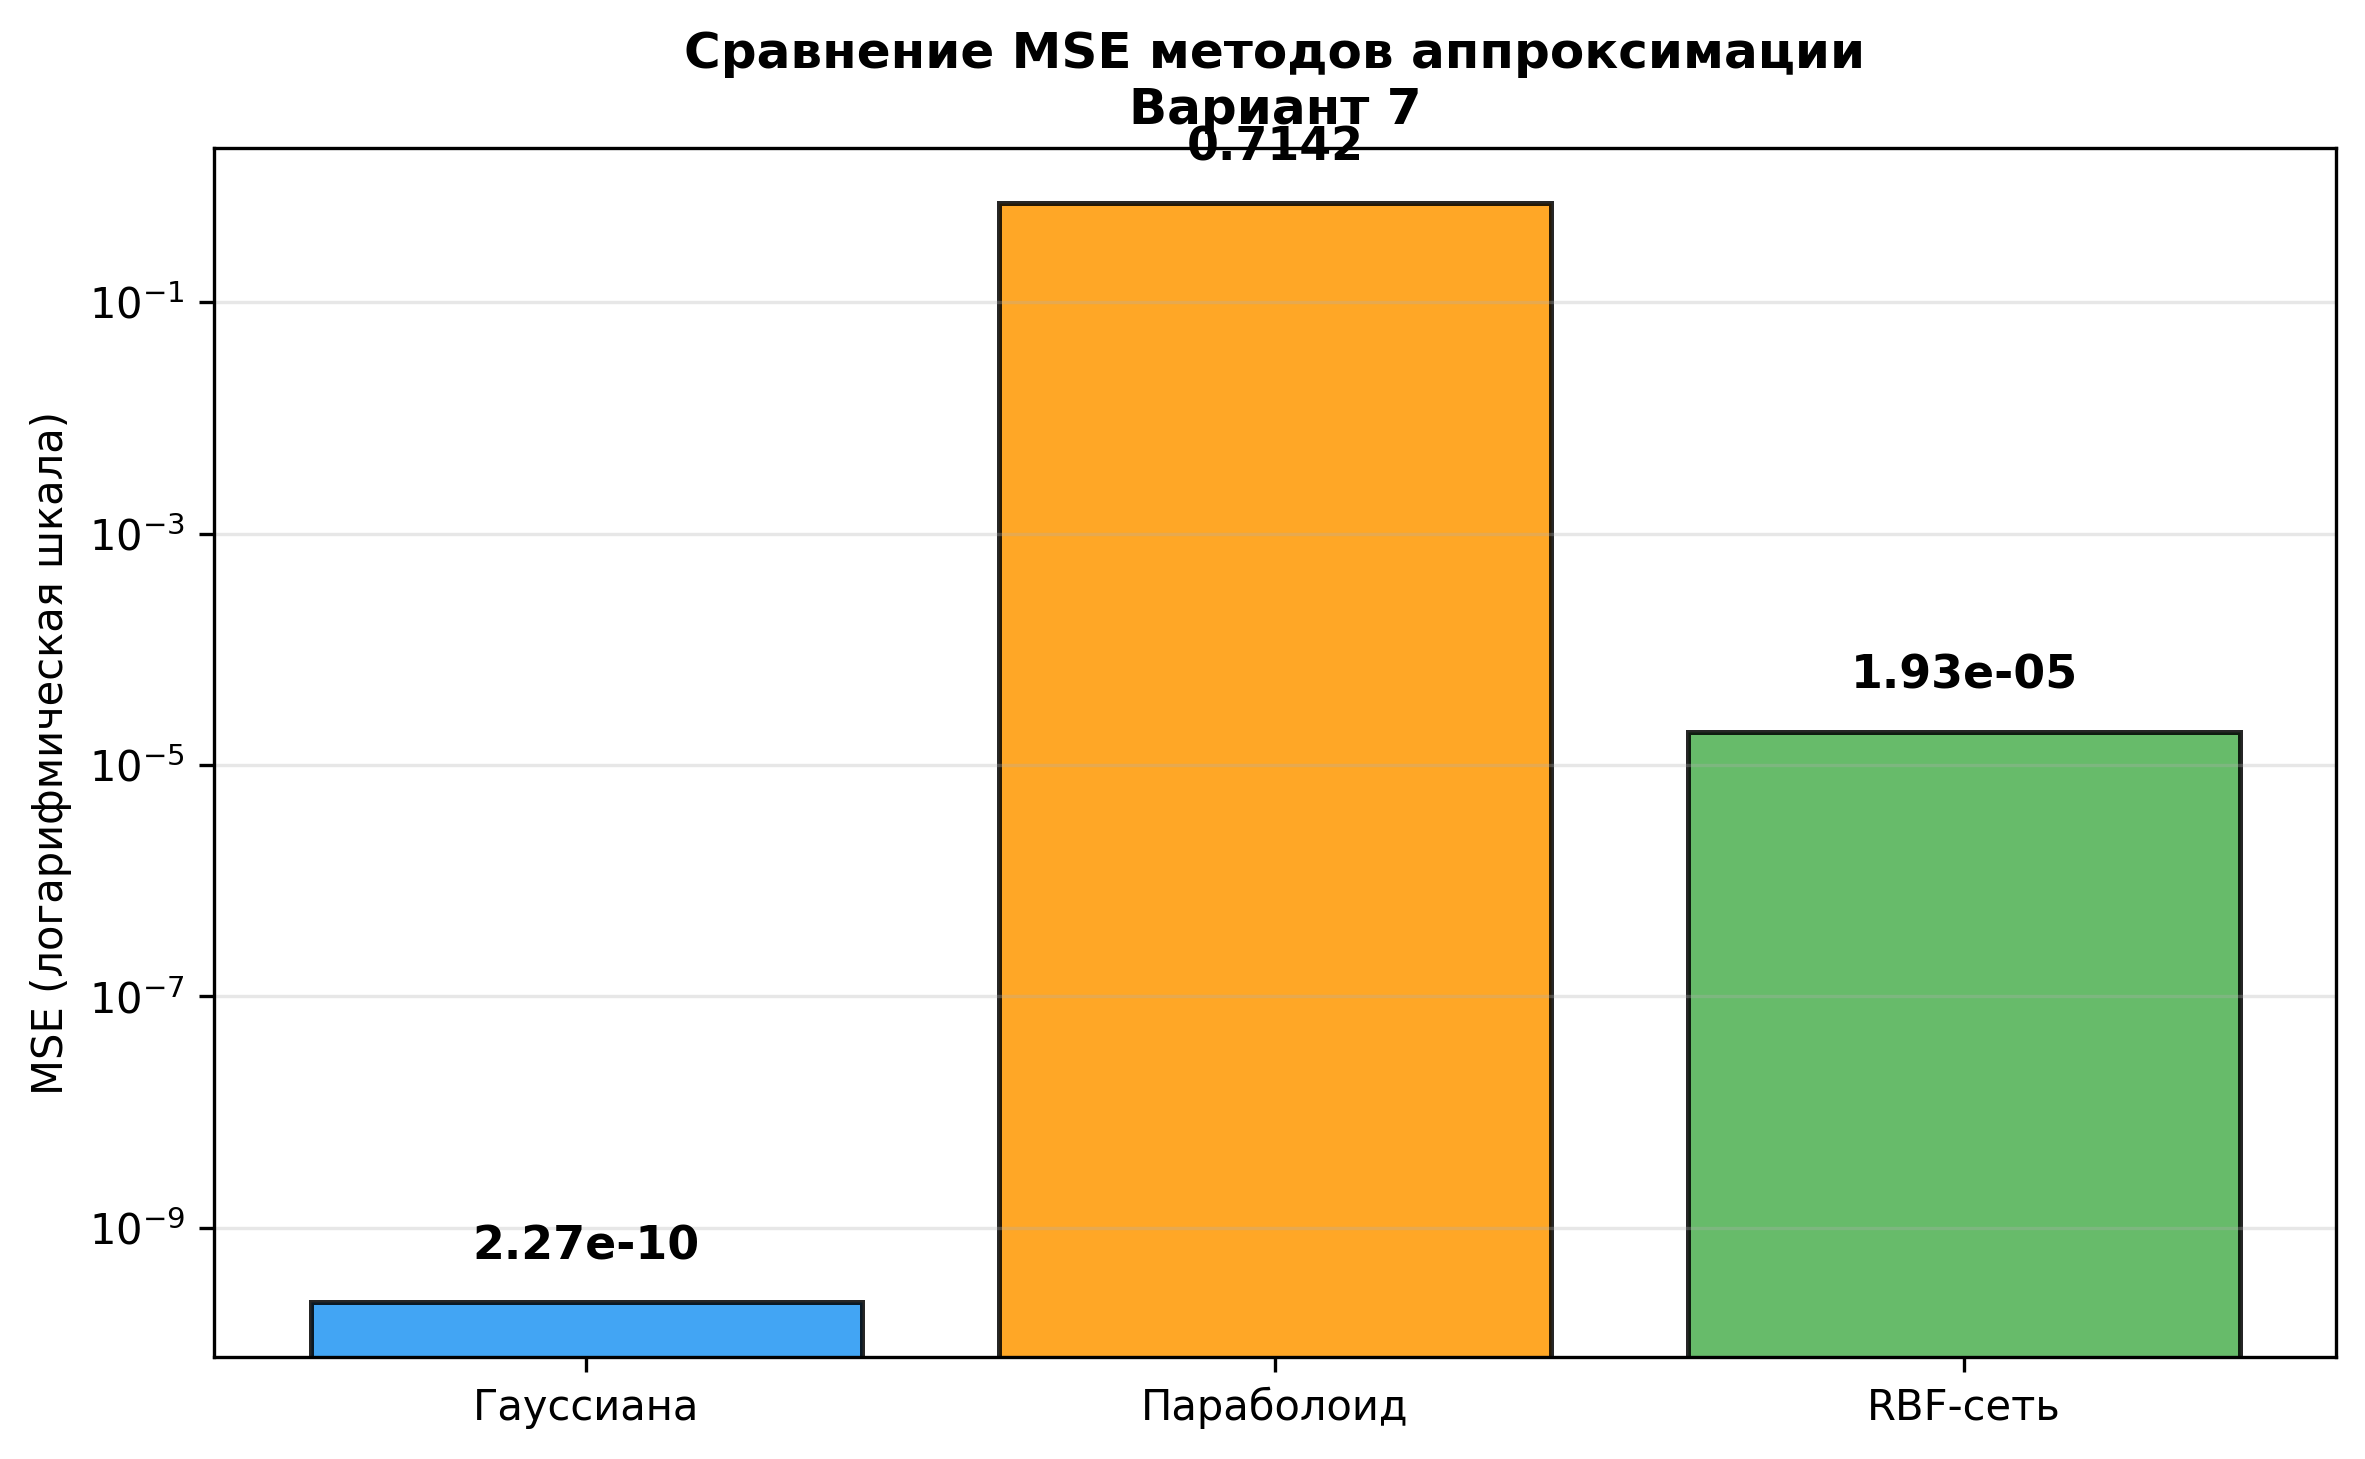
\includegraphics[width=0.8\textwidth]{pic/mse_comparison.png}
    \caption{Сравнение MSE трёх методов (логарифмическая шкала)}
    \label{fig:mse_comp}
\end{figure}

\begin{figure}[H]
    \centering
    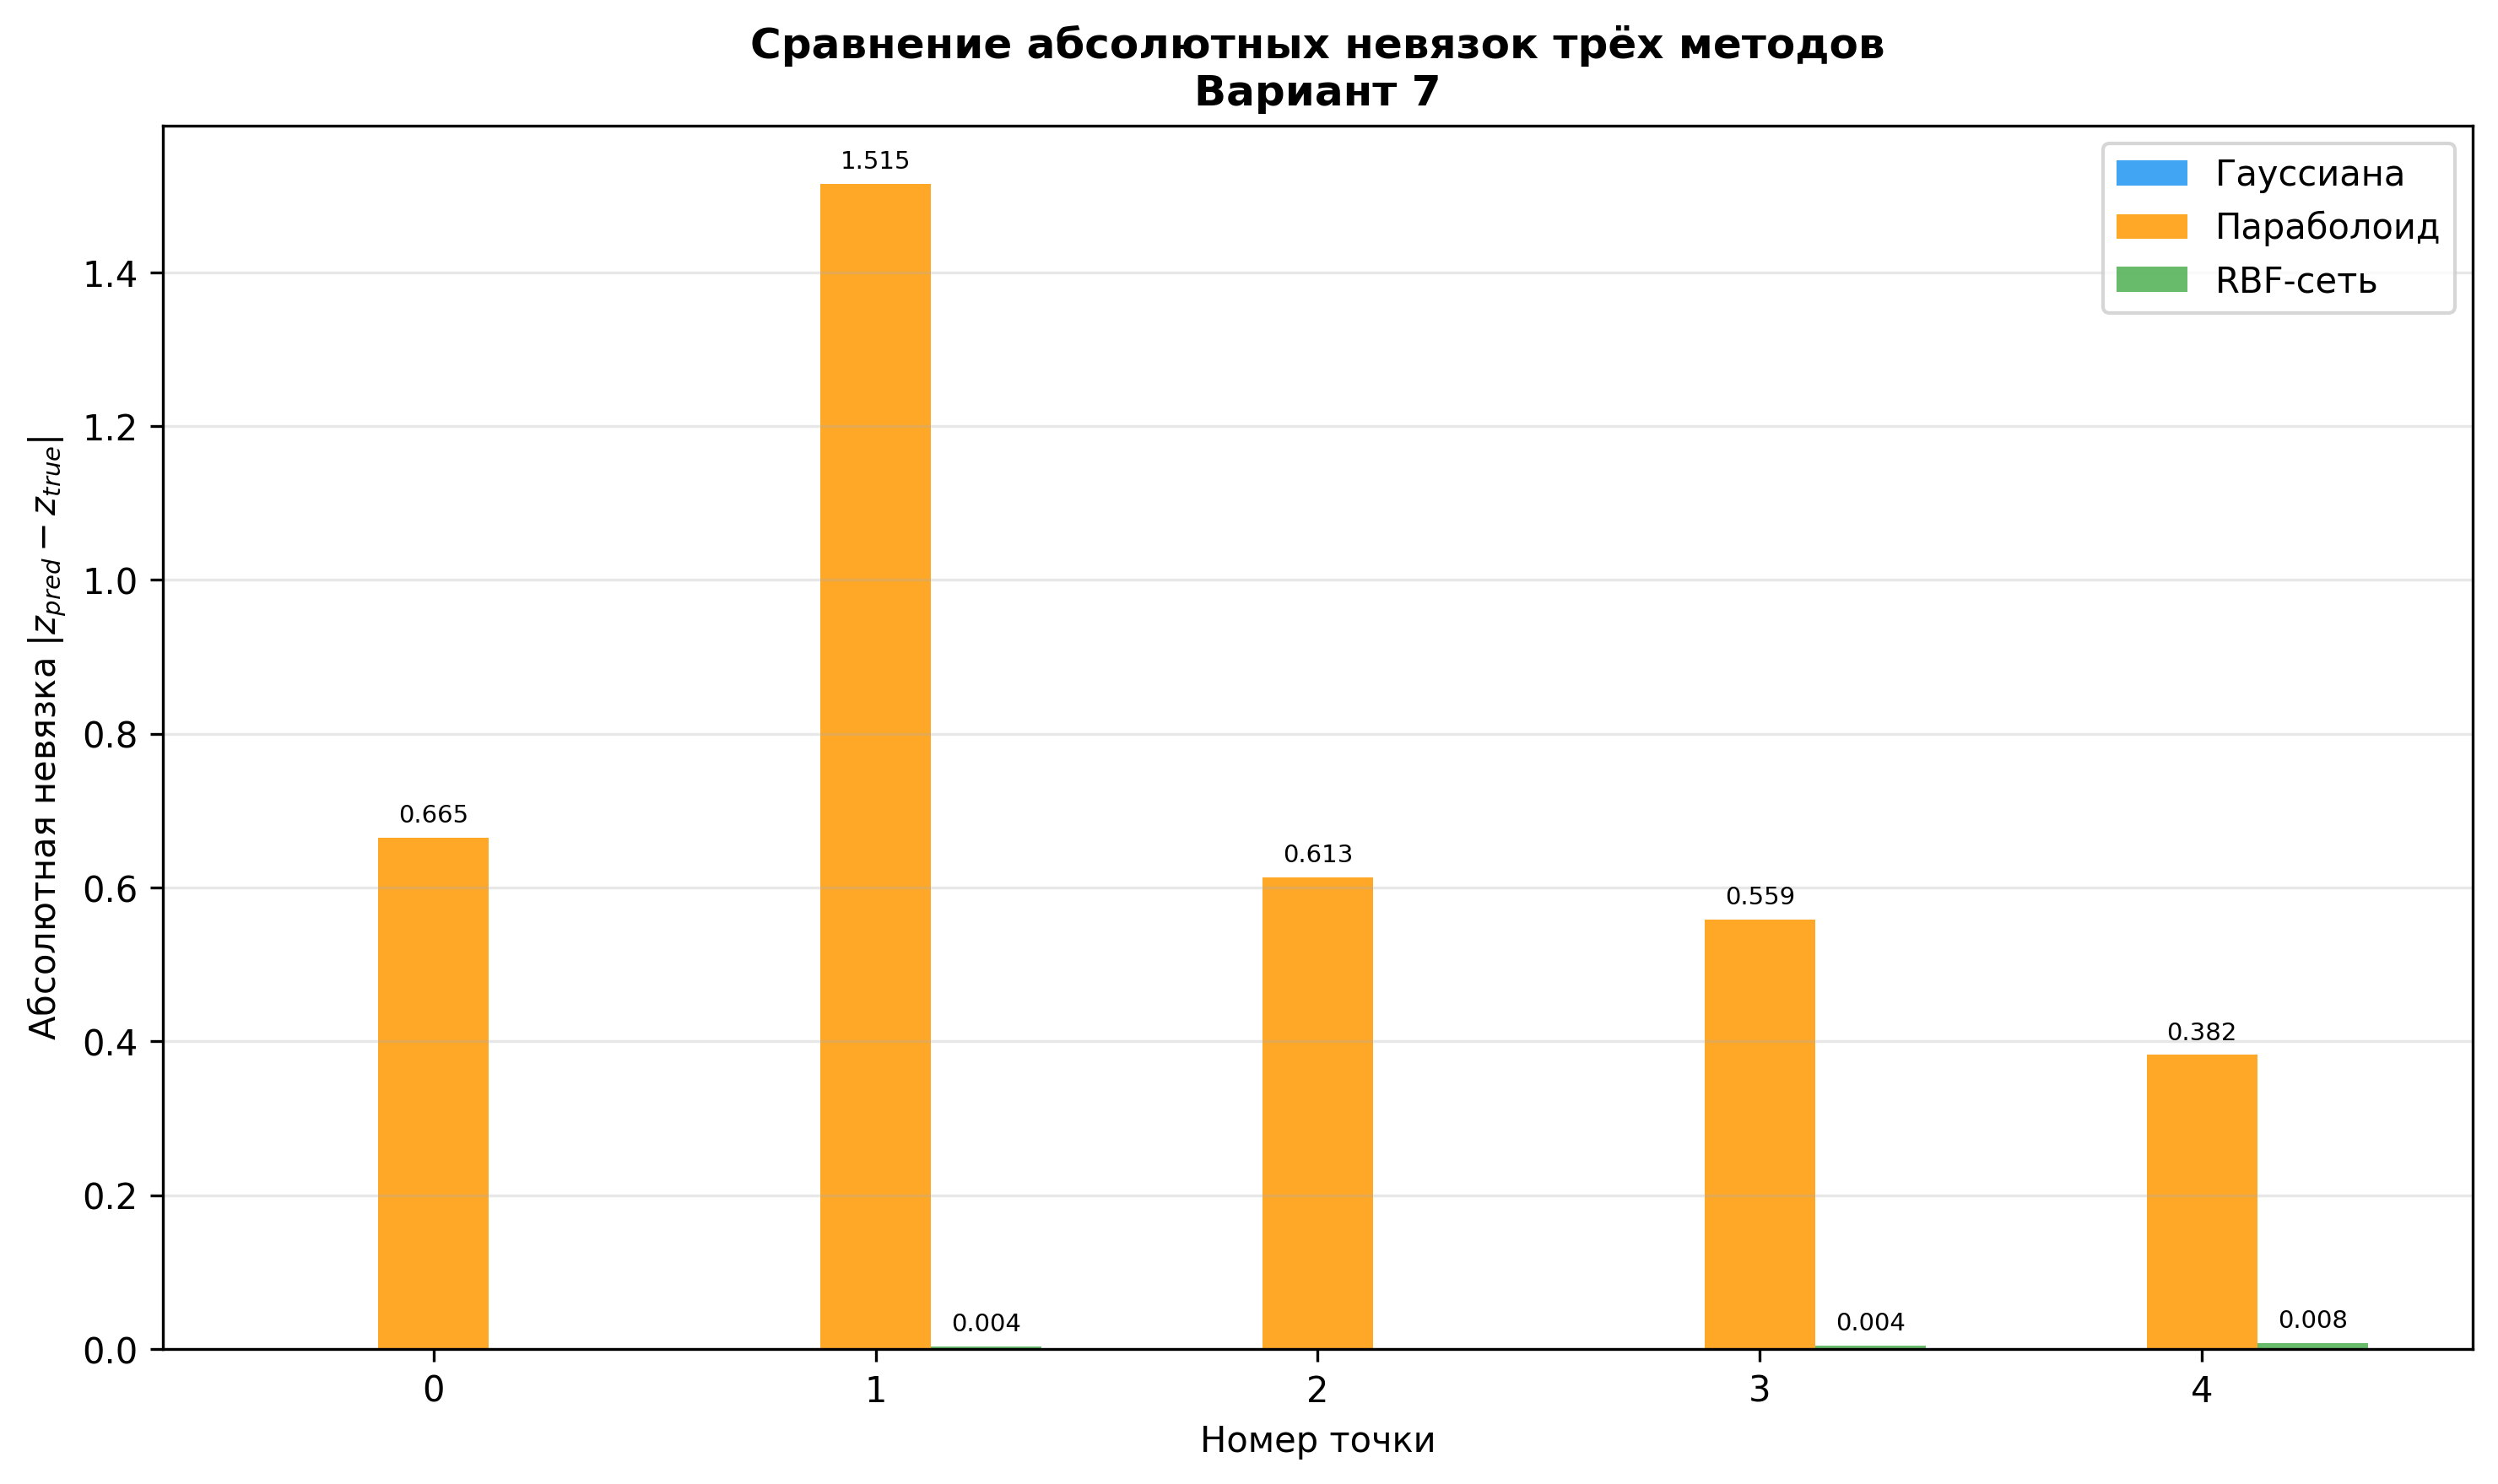
\includegraphics[width=0.85\textwidth]{pic/error_comparison.png}
    \caption{Абсолютные невязки по точкам для трёх методов}
    \label{fig:error_comp}
\end{figure}

\begin{figure}[H]
    \centering
    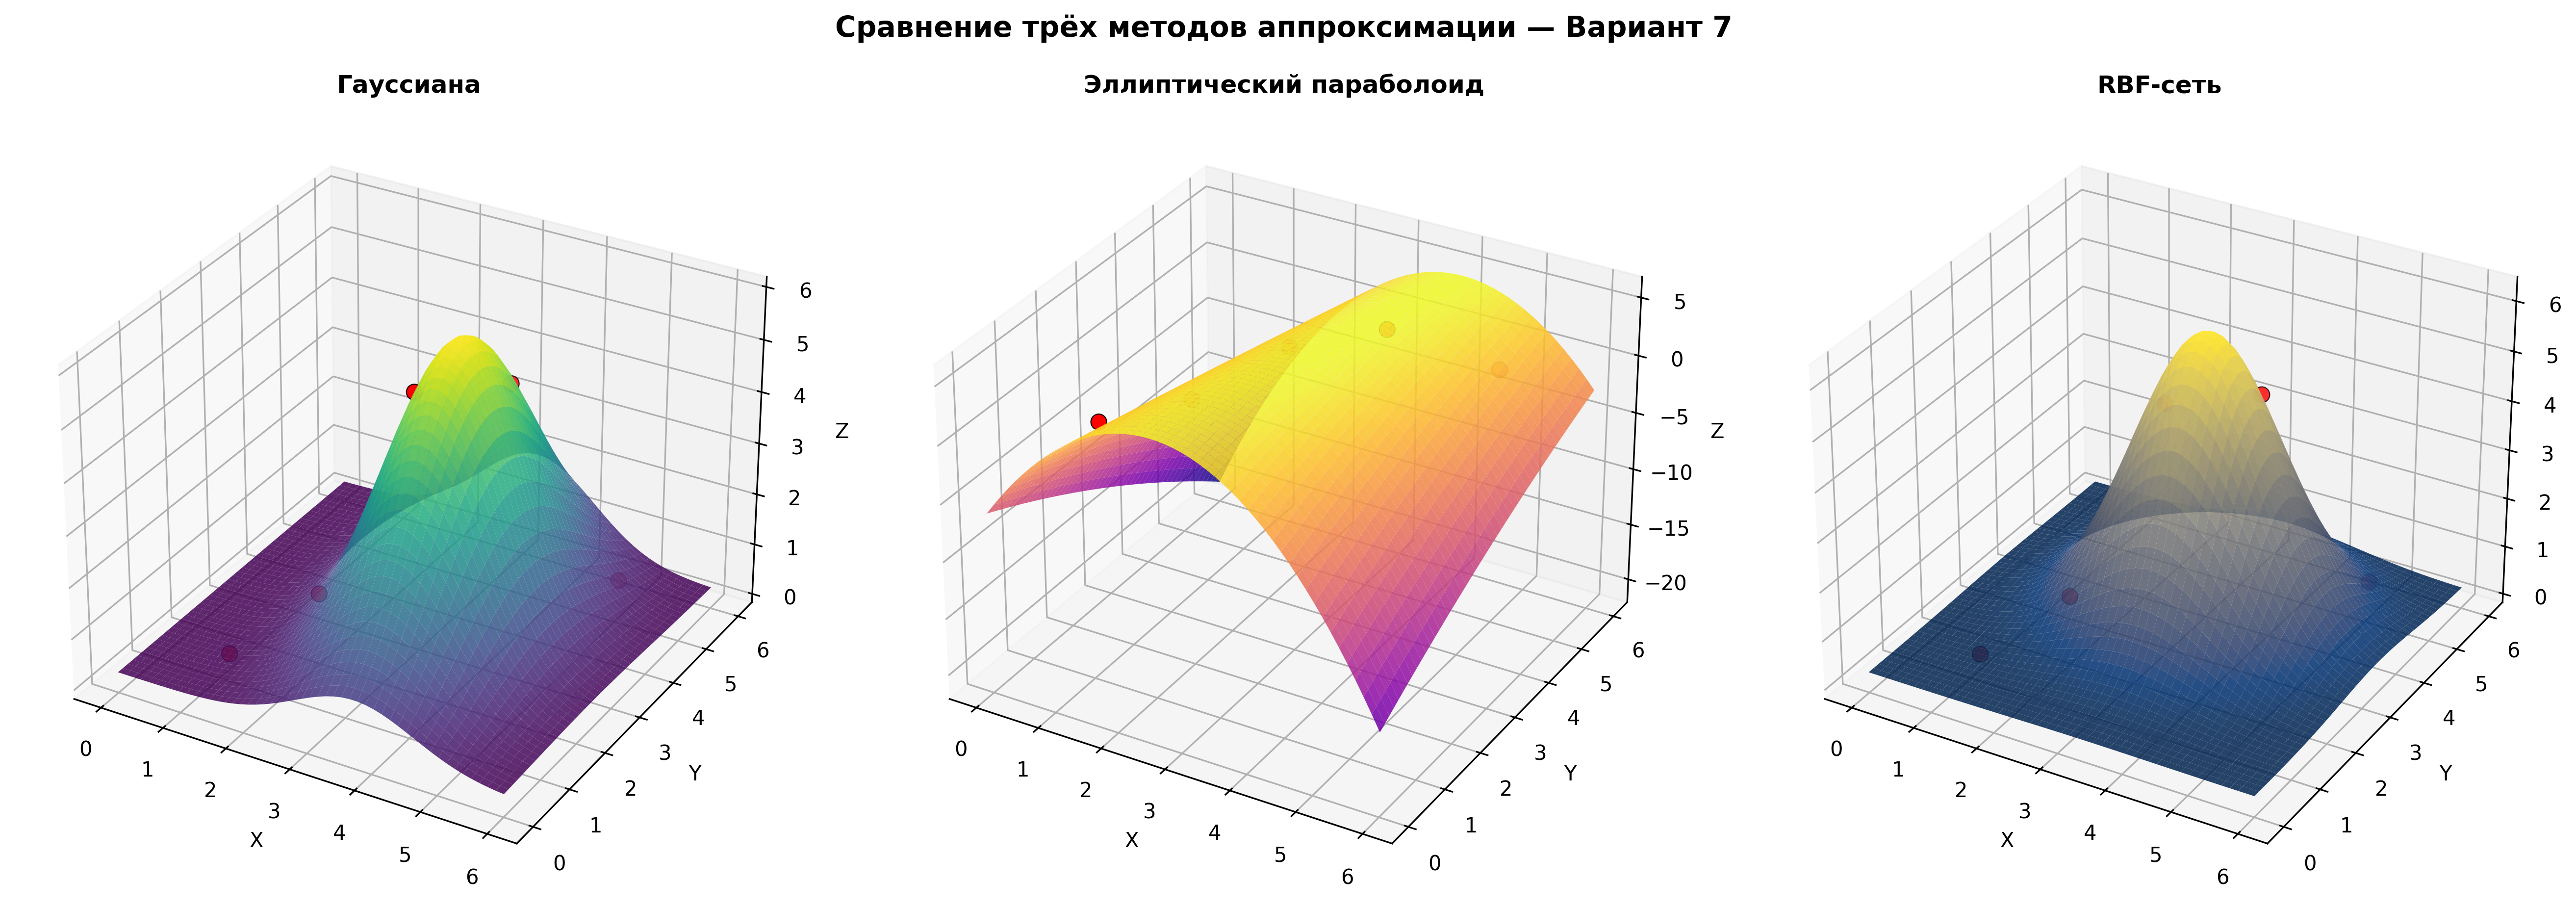
\includegraphics[width=\textwidth]{pic/all_models_3d.png}
    \caption{Сравнение 3D-поверхностей: Гауссиана (слева), Параболоид (центр), RBF-сеть (справа)}
    \label{fig:all_3d}
\end{figure}

\subsection{Анализ}

Результаты сравнения трёх методов можно интерпретировать следующим образом:

\begin{enumerate}
    \item \textbf{Гауссиана} ($\text{MSE} \approx 10^{-10}$) --- наилучшая модель. Данные были сгенерированы по гауссовому распределению, поэтому модель восстанавливает истинную зависимость с машинной точностью.

    \item \textbf{RBF-сеть} ($\text{MSE} \approx 10^{-5}$) --- также отличная аппроксимация. Будучи по сути суммой двух гауссиан, RBF-сеть нашла решение, где один нейрон моделирует основной пик (вес $\approx 5.82$), а второй имеет пренебрежимый вес ($\approx -0.006$). Несколько большая ошибка по сравнению с чистой гауссианой объясняется стохастической природой градиентного спуска.

    \item \textbf{Эллиптический параболоид} ($\text{MSE} = 0.7142$) --- непригоден для аппроксимации данных варианта 7. Причины:
    \begin{itemize}
        \item Параболоид с $a < 0, b < 0$ стремится к $-\infty$ при удалении от вершины, в то время как гауссиана асимптотически выходит на постоянный уровень $b = 0.2348$.
        \item Параболоид имеет постоянную кривизну, в то время как гауссиана имеет точку перегиба (S-образный профиль), которую квадратичная модель не может воспроизвести.
        \item Наибольшие невязки наблюдаются в точках 0 и 1 (края и промежуточная область), где расхождение между квадратичной и экспоненциальной формой максимально.
    \end{itemize}
\end{enumerate}

\subsection{Общие выводы}

\begin{enumerate}
    \item Для данных варианта 7 оптимальным методом аппроксимации является \textbf{двумерная гауссиана} (7 параметров, MSE $\approx 10^{-10}$). Модель физически интерпретируема: амплитуда А, центр пика $(x_0, y_0)$, ширины $\sigma_x, \sigma_y$, поворот $\theta$ и фоновый уровень $b$.

    \item \textbf{RBF-сеть} (9 параметров, MSE $\approx 10^{-5}$) даёт почти столь же хорошие результаты. Она является универсальным аппроксиматором и может применяться для данных произвольной формы, однако требует больше вычислительных ресурсов и настройки гиперпараметров (число нейронов, скорость обучения).

    \item \textbf{Эллиптический параболоид} не следует применять для аппроксимации колоколообразных функций. Его использование оправдано только тогда, когда данные заведомо имеют квадратичный характер.
\end{enumerate}
